\documentclass[a4paper,11pt]{article}

\parindent0cm
\usepackage
[backend=biber,style=apa,sorting=nyt]
{biblatex}
\addbibresource{literature.bib}

\usepackage{numprint}
\npthousandsep{\,}

\makeatletter
\newcommand\notsotiny{\@setfontsize\notsotiny{8}{8}}
\newcommand\micro{\@setfontsize\notsotiny{4.5}{4.5}}
\newcommand\middletiny{\@setfontsize\notsotiny{6}{6}}
\makeatother

\usepackage{float}
\usepackage{listofsymbols}
\usepackage[utf8]{inputenc}
\usepackage{csquotes}
\usepackage{array}
\usepackage{dirtytalk}
\usepackage{amsmath}
\usepackage{bm}
\usepackage{amssymb}
\usepackage{amsthm}
\usepackage{amsfonts}
\usepackage{color}
\usepackage{layouts}
% printing the textsize used
% \printinunitsof{cm}
% \prntlen{\textwidth}
\usepackage[usenames,dvipsnames]{xcolor}
\usepackage{tabularx}
\usepackage{graphicx}
\usepackage{pdfpages}
\usepackage[ngerman]{babel}
\usepackage[left=3cm,right=2.5cm,top=2cm,bottom=2cm]{geometry}
\renewcommand{\baselinestretch}{1.5}\normalsize % Zeilenabstand 1.5



\begin{document}








\section{Einleitung}

\begin{itemize}
\item Natural Language Processing (NLP) ist aktuelles Thema mit vielen Anwendungsfällen, zB. überwachte Klassifikation von Kurztexten.
   \item Größtenteils Artikel und Tutorials über binäre Klassifikation (zB. IMDB Sentiment Classification, Spam Vs NonSpam etc.)
   \item In der Realität oft viel mehr Klassen, zB:
   \item Themen-Kategorisierung von Kundenbeschwerden
   \item Tagging von Forenbeiträgen (Stackoverflow)
   \item Produktkategorien von Artikeln anhand Artikelbeschreibung
   \item Kategorisierung von Nachrichtenkategorien
    \item nutzen der klassifikation für die Redaktion
    \item oft nur binäre klassifikation, multi selteneres topic
    \item Multiclass auch bei next best offer
    \item bag of words kein guten Ruf, bei welchen Datensätzen lohnen sich Neural nets überhaupt.
\end{itemize}{}



\section{Datensatz und Problemstellung}

In diesem Kapitel wird der für diese Thesis relevante Datensatz vorgestellt. Nach dessen Bereinigung erfolgt eine Exploration und anschließend die Darlegung der Zielstellung dieser Thesis.


\subsection{Initialer Datensatz}

Der Datensatz trägt den Titel \textit{News Category Dataset} (\cite{dataset}) und stammt von der Machine Learning Plattform \textit{Kaggle}. Er umfasst \numprint{200853} Beobachtungen, die Informationen in englischer Sprache über Artikel der US-Amerikanischen Onlinezeitung \textit{Huffpost} enthalten. Der Zeitraum, in dem die Veröffentlichungen stattgefunden haben, erstreckt sich vom 28.01.2012 bis zum 25.05.2018, also über eine Zeitspanne von über $6$ Jahren. Die Inhalte der Artikel sind lediglich verlinkt und nicht direkt im Datensatz enthalten. Für jeden Artikel ist die Nachrichtenschlagzeile des Artikels angegeben. Zusätzlich zu dem Link des Artikels ist für jeden Datenpunkt das Veröffentlichungsdatum, der Name des Autors, eine Kurzbeschreibung und die Nachrichtenkategorie gegeben. Letzteres ist die Zielvariable (genauere Erläuterung in Kapitel \ref{Kap:Zielst}), die $41$ verschiedene Ausprägungen annimmt. Die Kurzbeschreibung enthält ähnliche Informationen wie die Nachrichtenüberschrift und ist nur teilweise vorhanden. Für die Beantwortung der Fragestellung (Kapitel \ref{Kap:Zielst}) soll nur die Schlagzeile als unabhängige Variable in die Modellierung eingehen. Bevor eine Exploration des Datensatz erfolgt, werden im nächsten Abschnitt vorgenommene Änderungen an den relevanten Variablen Nachrichtenkategorie und Nachrichtenschlagzeile aufgelistet und begründet.


\subsection{Änderungen am Datensatz} \label{kap:2_2Aend}

In der englischen Sprache spielt die Groß- und Kleinschreibung außer bei der Nutzung von Personalpronomen keine Rolle. Deshalb werden in den Texten alle Großbuchstaben zu Kleinbuchstaben konvertiert. Auf diese Weise werden in der Modellierung beispielsweise die Wörter \textit{Teacher} und \textit{teacher} nicht unterschiedlich behandelt. \\
\\
Die Artikel wurden vermutlich von einigen Autoren in unterschiedlichen Ländern geschrieben, denn die Texte enthalten unterschiedliche Zeichensätze. Bei der verwendeten \texttt{Utf8} Enkodierung entstanden bei unbekannten Zeichen Konvertierungsfehler (z.b. der Form \say{a@S}). Diese wurden durch Leerzeichen ersetzt. In dem Wissen, dass die Wörter des Textkorpus mit den \textit{Global Word Vectors} (Kapitel \ref{Kap:Glove}) abgeglichen werden, wurden einige Begriffe so ersetzt, dass bestimmte Wörter in den \textit{Global Word Vectors} gefunden werden. Zuerst erfolgte eine Entfernung von Sonderzeichen wie beispielsweise \say{©} oder \say{™}. Dann folgte die Ersetzung von Verneinungen wie zum Beispiel \say{n't} durch \say{ not}. Analog wurden \say{'ll} durch \say{ will} und \say{'ve} durch \say{ have} ersetzt. Kurzformen der Form \say{here's} wurden zu \say{here is} geändert, da sonst die Wörter mit Endung \say{'s} so als eigenständige Wörter repräsentiert werden und nicht sinngemäß als Tupel. Häufig vorkommende Eigennamen mit analoger Endung \say{trump's} wurden durch \say{trump his} ausgetauscht. Nachdem Vorkommnisse der Art \say{here's} entfernt wurden, können nun Vorkommnisse der Art \say{john's son} durch \say{john its son} ersetzt werden. So ist bei Wörtertupeln dieser Art zwar nicht das Geschlecht von John bekannt, aber zumindest offensichtlich, dass der Sohn John zugehörig ist. Nach der Bereinigung des Textkorpus wurden letztendlich noch $6$ Schlagzeilen entfernt, die keine Wörter mehr enthalten. Es verbleiben nun also insgesamt \numprint{200847} Beobachtungen.\\
\\
Nach der umfangreichen Bereinigung des Schlagzeilen-Textkorpus liegt nun die Zielvariable Nachrichtenkategorie im Fokus.
Bei genauerer Betrachtung der $41$ Kategorien fällt auf, dass diese teilweise bereits namentlich sehr ähnlich ausfallen. In Tabelle \ref{tab:parentsMerge} sind beispielhaft $4$ Schlagzeilen der Kategorien \textit{parents} und \textit{parenting} aufgeführt.

\begin{table}[ht]
\begin{center}
\begin{tabular}{ | p{0.1 \textwidth} | p{0.42 \textwidth}| p{0.42 \textwidth} | }
  \hline
Beispiel & Kategorie \textit{parents}  & Kategorie \textit{parenting} \\ 
  \hline
1 & 40 tweets that sum up life with 4-year-olds & a baby book of disasters \\ 
  2 & these were the trendiest baby names in the late '80s & it is time to find your tribe \\ 
  3 & these quotes from kids are hilarious, adorable and oddly insightful & help huffpost parents win a webby award! \\ 
  4 & 30  'star wars'-inspired names parents are giving their babies & why our 'imperfect' moments are perfect to our children \\ 
   \hline
\end{tabular}
\caption{Beispiele für Schlagzeilen der Kategorien \textit{parents} und \textit{parenting}}
\label{tab:parentsMerge}
\end{center}
\end{table}

Anhand der Beispiele wird deutlich, dass es schwierig ist, diese mit menschlicher Intuition eine der beiden Kategorien eindeutig zuzuordnen. Als zusätzlicher Indikator, der für die Verschmelzung zweier Kategorien spricht, erfolgte die Betrachtung der relativen Schnittmenge der gemeinsamen häufigsten Wörter. Die häufigsten Wörter pro Kategorie werden ermittelt, indem die kompletten Daten auf die entsprechende Kategorie gefiltert werden. Anschließend werden Symbole und \textit{Stopwords} (Wörter wie \say{he}, \say{is} oder \say{through}, die komplette Liste ist in Tabelle \ref{appendix:Stopwords} im Anhang zu finden) entfernt und die Wörter nach der gesamten Anzahl ihres Auftretens sortiert. Tabelle \ref{tab:categoryMerge} zeigt die relative Schnittmenge der $100$ häufigsten Wörter für einen Ausschnitt der Paare an Kategorien.

\begin{table}[ht]
\begin{center}
\begin{tabular}{|l|l|c|c|}
  \hline
Kategorie 1 & Kategorie 2  & relative Schnittmenge & neue Kategorie\\
  \hline
\textit{healthy living} & \textit{wellness} & 0.76 & \textit{wellness \& healthy living} \\ 
  \textit{parents} & \textit{parenting} & 0.74 & \textit{parents} \\ 
  \textit{taste} & \textit{food \& drink} & 0.70 & \textit{food, drink \& taste}\\ 
  \textit{world news} & \textit{the worldpost} & 0.68 & \textit{world news}\\ 
  \textit{arts} & \textit{culture \& arts} & 0.60 & \textit{arts \& culture}\\ 
  \textit{style} & \textit{style \& beauty} & 0.58 & \textit{style \& beauty} \\ 
  \textit{the worldpost} & \textit{worldpost} & 0.58 & \textit{world news}\\ 
  \textit{world news} & \textit{worldpost} & 0.55 & \textit{world news}\\ 
  \textit{green} & \textit{environment} & 0.53 & \textit{green \& environment}\\ 
  \textit{fifty} & \textit{parenting} & 0.50 & -\\ 
    \vdots & \vdots & \vdots & -\\
  \textit{parents} & \textit{fifty} & 0.48 & - \\ 
  \textit{arts \& culture} & \textit{arts} & 0.46 & \textit{arts \& culture}\\  
  \vdots & \vdots & \vdots & -\\
  \textit{world news} & \textit{home \& living} & 0.05 & - \\ 
  \textit{crime} & \textit{food \& drink} & 0.04 & -\\
  \hline 
  \hline 
  \multicolumn{2}{|c|}{Mittelwert} &  0.24 & \\
   \hline
\end{tabular}
\caption{Relative Schittmenge der $100$ häufigsten Wörter für ausgewählte Paare an Kategorien, absteigend geordnet nach der relativen Schnittmenge.}
\label{tab:categoryMerge}
\end{center}
\end{table}

Die ersten $10$ Zeilen von Tabelle \ref{tab:categoryMerge} beinhalten Kategorien, die eine relative Schnittmenge der gemeinsamen Wörter von $0.50$ oder höher haben. In den letzten beiden Zeilen ist zu sehen, dass inhaltlich verschiedene Kategorien eine vergleichbar geringe Schnittmenge an häufigsten Wörtern haben. Im Mittel hat ein Paar an Kategorien eine gemeinsame Schnittmenge von $0.24$. Dieser Wert wirkt hoch, da \textit{Stopwords} und Sonderzeichen bereits entfernt wurden.
Die Grenze, ab der $2$ Kategorien zusammengelegt werden, wird bei einer Überschneidung von $50$ Prozent angesiedelt. Es werden dennoch $2$ Ausnahmen gebildet. \textit{parents} und \textit{fifty} werden nicht zusammengelegt. Außerdem wird das Paar \textit{arts \& culture} und \textit{arts} mit einer Überschneidung von $0.46$ zusammengelegt, da bereits \textit{arts} und \textit{culture \& arts} mit einer Überschneidung von $0.60$ fusioniert wurden.\\
Mit den Argumenten der menschlichen Intuition und der Ergebnisse aus Tabelle \ref{tab:categoryMerge} wurden in folgenden Fällen die Kategorien zusammengelegt:
Die Kategorien \textit{healthy living} und \textit{wellness} wurden zu \textit{wellness \& healthy living}; \textit{parents} und \textit{parenting}  zu \textit{parents}; \textit{taste} und \textit{food \& drink} zu \textit{food, drink \&taste}; \textit{arts}, \textit{culture \& arts} und \textit{arts \& culture} zu \textit{arts \& culture}; \textit{the worldpost}, \textit{worldpost} und \textit{world news} zu \textit{world news}; \textit{style} und \textit{style \& beauty} zu \textit{style \& beauty};  sowie \textit{green} und \textit{environment} zu \textit{green \& environment}. Die $41$ Kategorien wurden somit auf $32$ Kategorien reduziert, welche inhaltlich mit menschlicher Intuition unterscheidbar sind. Nach den Modifikationen folgt im nächsten Abschnitt eine Exploration des Datensatzes.

\subsection{Exploration des bereinigten Datensatzes}\label{kap:exploration}

Von großem Interesse ist die Verteilung der Nachrichtensparten im kompletten bereinigten Datensatz.
Abbildung \ref{abb:barplotCategories} zeigt die absoluten Anzahlen der Datenpunkte pro Nachrichtenkategorie. 

\begin{figure}[ht]
    \centering
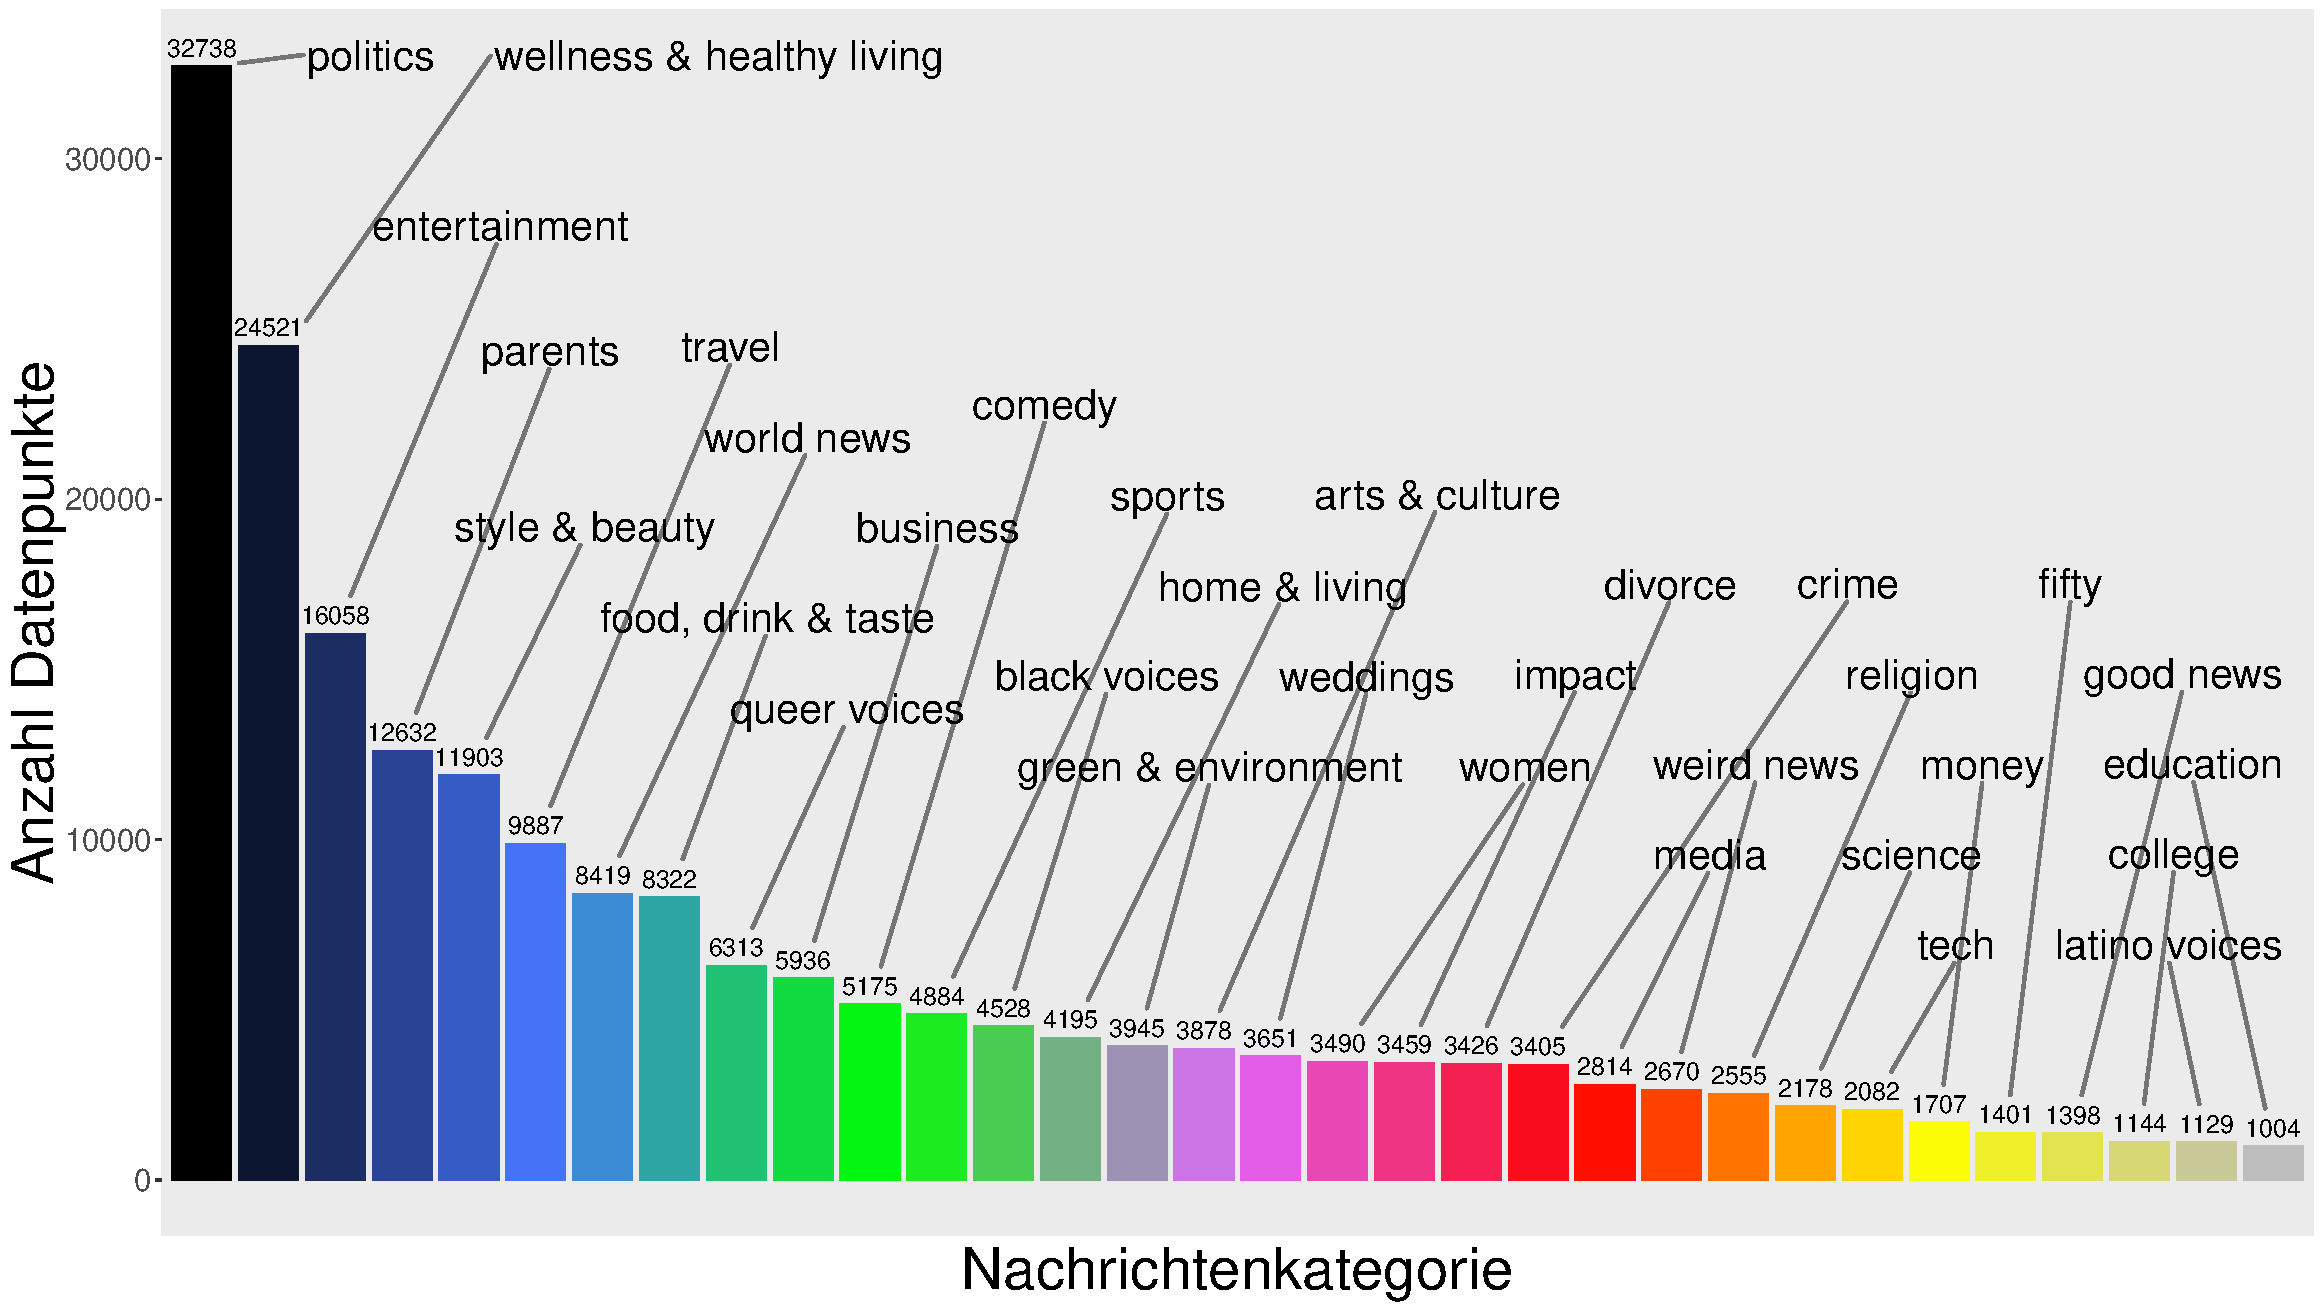
\includegraphics[width = \textwidth,  keepaspectratio]{Images/barplotCategories.pdf} 
\caption{Anzahl Datenpunkte pro Nachrichtenkategorie}
\label{abb:barplotCategories}
\end{figure}

Es ist festzustellen, dass die Kategorien keineswegs ausgeglichen vorliegen. Die häufigste Kategorie stellt \textit{politics} dar mit $\numprint{32738}$ Datenpunkten. Zweit- und dritt-häufigste Kategorien sind \textit{wellness \& healthy living} und \textit{entertainment} mit $\numprint{24521}$ und $\numprint{16058}$ Beobachtungen. Die Nachrichtensparten mit den wenigsten Artikeln bilden \textit{college}, \textit{latino voices} und \textit{education} mit $\numprint{1144}$, $\numprint{1129}$ und $\numprint{1004}$ Beobachtungen.\\
Die ersten $6$ Kategorien stellen bereits $53.6$ Prozent der gesamten Beobachtungen dar. Durchschnittlich beinhaltet eine Kategorie $\numprint{6276.47}$ Nachrichtenschlagzeilen.\\
\\
Es folgt nun eine gesamtheitliche Exploration des Textkorpus der Schlagzeilen. Im Rahmen der Analyse zählen Symbole sämtlicher Art auch als Wörter. Die kürzeste Überschrift des Datensatzes enthält nur $1$ Wort, während die längste $82$ Wörter umfasst. Durchschnittlich enthält eine Artikel-Schlagzeile $11.022$ Wörter. Das Vokabular aller Schlagzeilen umfasst $\numprint{58717}$ Wörter, wobei \say{the} das häufigste Wort ist und in $\numprint{54139}$ Artikelüberschriften vorkommt. $\numprint{24372}$ Wörter kommen nur einmal vor. In der Betrachtung der mittleren Wortanzahlen pro Kategorie fällt auf, dass diese differieren. Die Kategorie mit der höchsten durchschnittlichen Anzahl von $12.724$ Wörtern ist \textit{style \& beauty}. Die Kategorie, bei der sich die Autoren durchschnittlich am kürzesten fassen, ist \textit{wellness \& healthy living} mit $9.367$ Wörtern. Eine weitere interessante Fragestellung ist, ob in den Kategorien bestimmte Sonderzeichen oder Symbole besonders häufig oder selten vorkommen. Abbildung \ref{abb:barplotSymbols} zeigt die relative Anzahl der Vorkommnisse verschiedener Symbole in den Schlagzeilen pro Kategorie.

\begin{figure}[ht]
    \centering
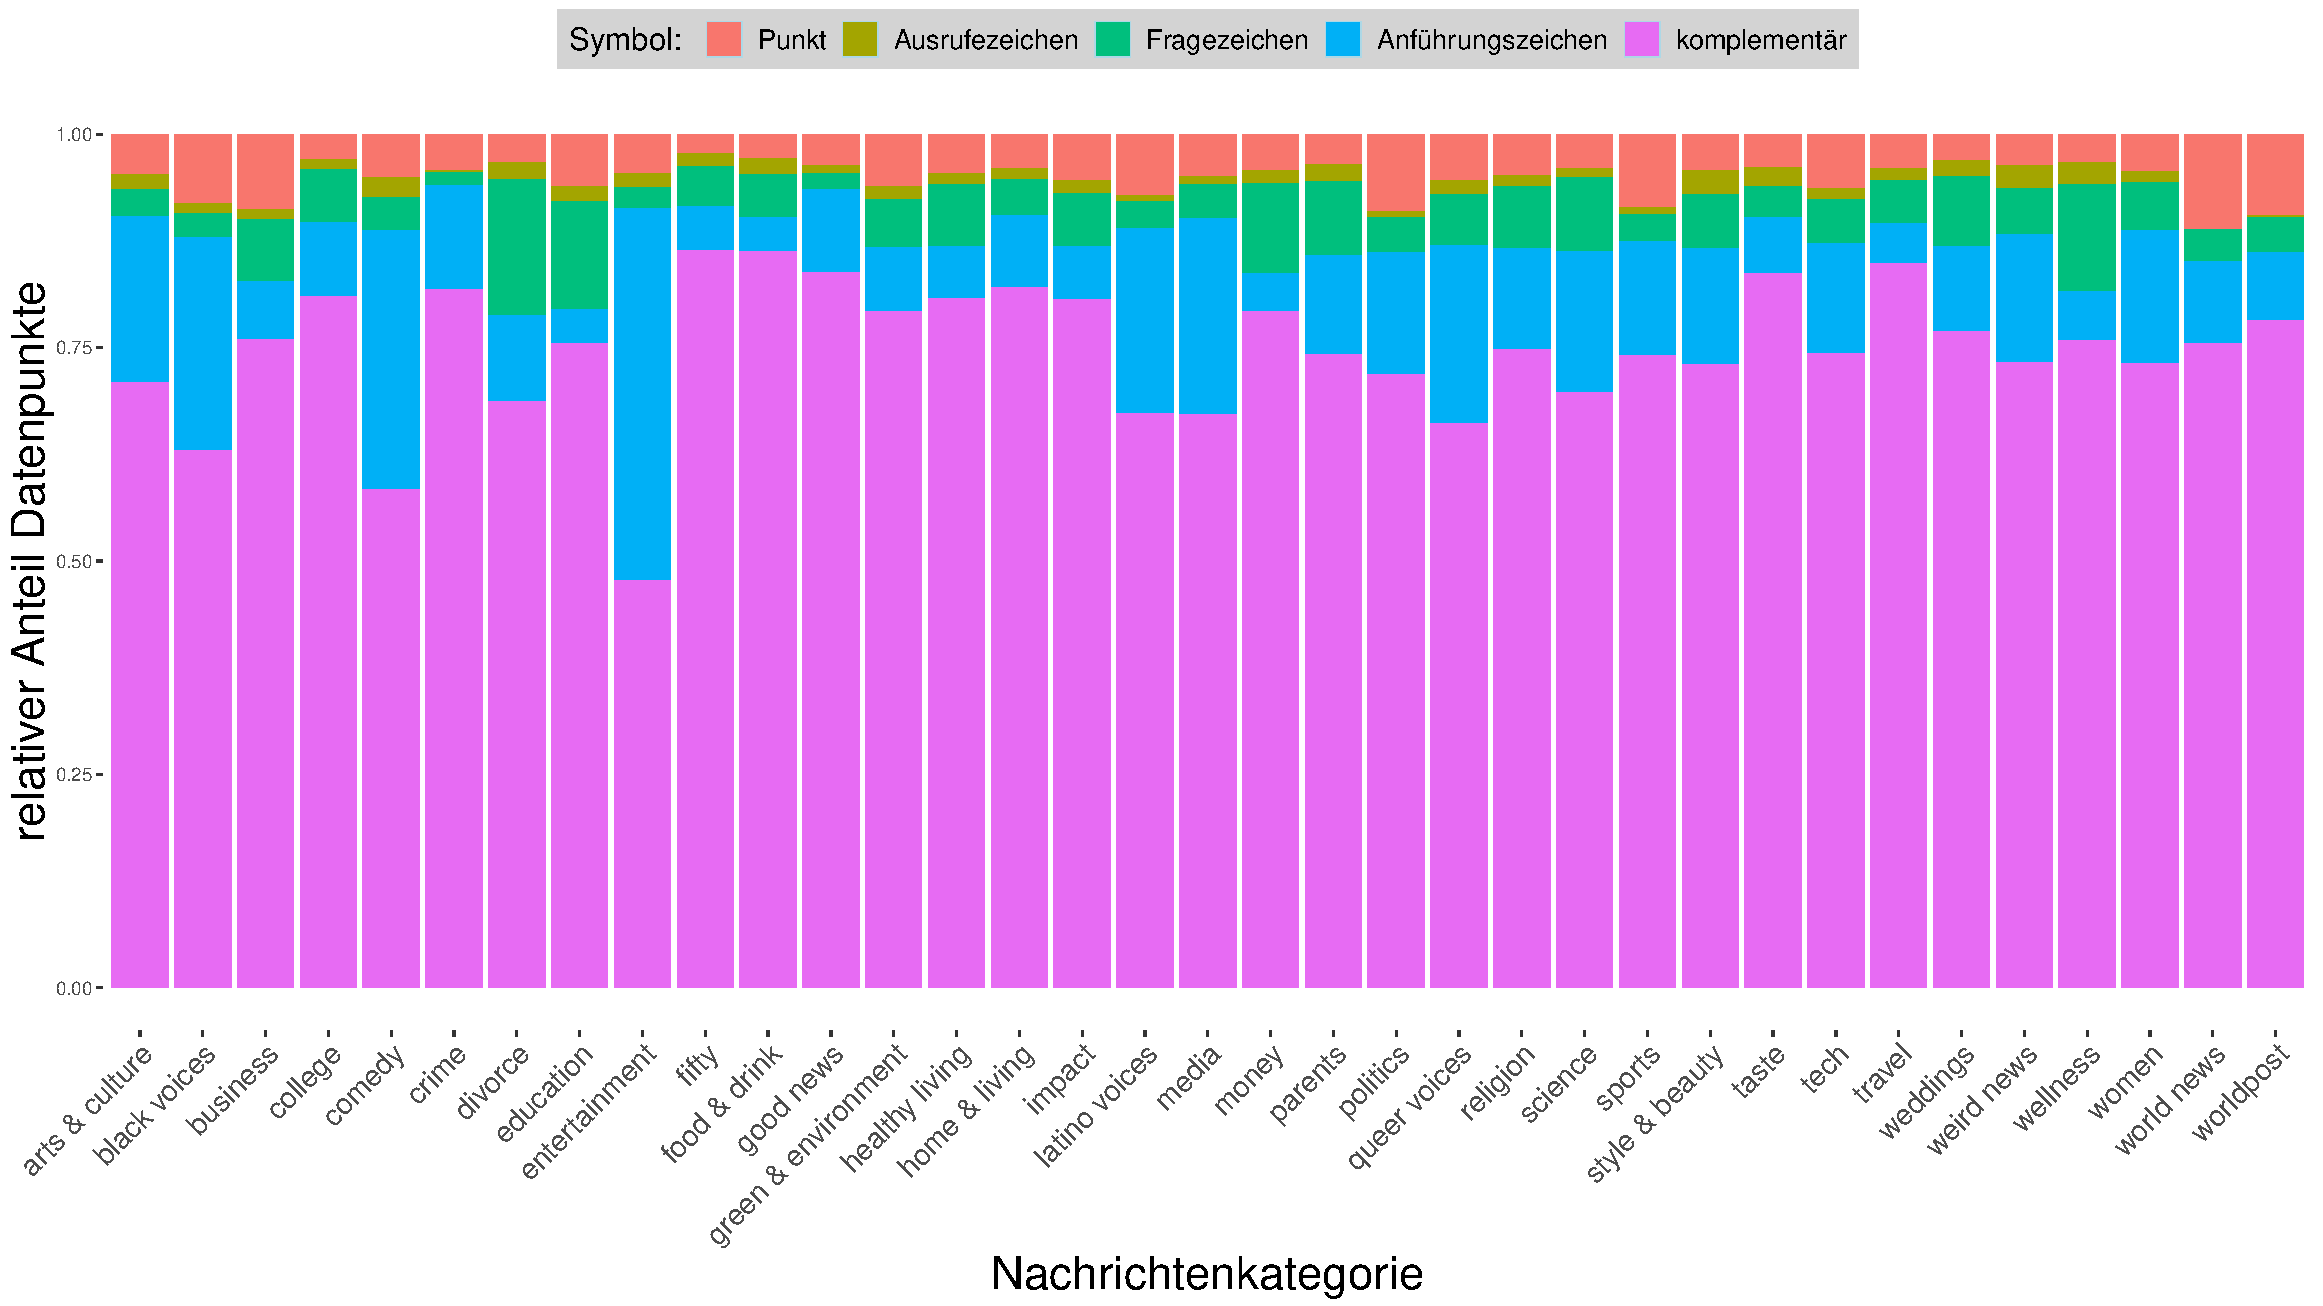
\includegraphics[width = \textwidth,  keepaspectratio]{Images/barplotSymbols.pdf} 
\caption{Relativer Anteil Datenpunkte für ausgewählte Sonderzeichen pro Kategorie. Der komplementäre Anteil ist der Anteil Datenpunkte, in dem keine der aufgeführten Sonderzeichen enthalten sind.}
\label{abb:barplotSymbols}
\end{figure}

Ein Wert von beispielsweise $0.15$ für eine bestimmte Nachrichtensparte in der Grafik ist so zu interpretieren, dass in $15$ Prozent aller Schlagzeilen dieser Kategorie das entsprechende Symbol mindestens einmal aufgetaucht ist. Die im Folgenden beschriebenen Durchschnitte sind Mittelwerte pro Kategorie und werden nicht über den gesamten Datensatz berechnet. Betrachtet sei nun das Vorkommen eines Punktes in einer Schlagzeile. Dieses kann so interpretiert werden, dass eine Schlagzeile mehrere Sätze enthält. Dies ist insgesamt mit einem durchschnittlichen relativen Anteil von $0.050$ selten der Fall. In der Sparte \textit{world news} kommen mehrere Sätze mit $0.098$ am häufigsten vor, in \textit{fifty} mit $0.021$ am wenigsten. Der Mittelwert für Ausrufezeichen beträgt $0.015$ und die Kategorie \textit{style \& beauty} nimmt das Maximum mit $0.028$, die Kategorie \textit{world news} das Minimum mit $0.002$ an. Fragezeichen kommen in durchschnittlich $0.059$ der Schlagzeilen vor, dabei am häufigsten in \textit{divorce} mit $0.159$ und am seltensten mit $0.015$ in \textit{crime}. Anführungszeichen sind mit durchschnittlich $0.133$ von den hier betrachteten Satzzeichen am meisten vertreten. Sie wurden besonders oft mit $0.437$ in der \textit{entertainment} Sparte genutzt und kamen am seltensten mit $0.040$ in \textit{education} zum Einsatz. Die Rubrik \say{komplementär} gibt an, zu welchem relativen Anteil keines der betrachteten Symbole vorkommt. Durchschnittlich enthalten $0.743$ der Kategorien keine der hier betrachteten Sonderzeichen. Hier ist zu sehen, dass Kategorien wie \textit{entertainment}, \textit{comedy}, \textit{black voices} oder \textit{divorce} häufig Symbole beinhalten, die einen dramatischen Charakter ausdrücken. Sparten wie \textit{fifty}, \textit{food, drink \& taste} und \textit{travel} bleiben mit wenig Symbolen sachlicher. Abbildung \ref{abb:barplotSymbols} zeigt insgesamt, dass Symbole für die Kategorisierung der Nachrichtensparten wichtig sind und im Rahmen der in Kapitel \ref{Kap:Tfidf} beschriebenen \textit{Bag-Of-Words} und \textit{TFIDF} Methoden nicht entfernt werden sollten.

\begin{figure}[ht]
    \centering
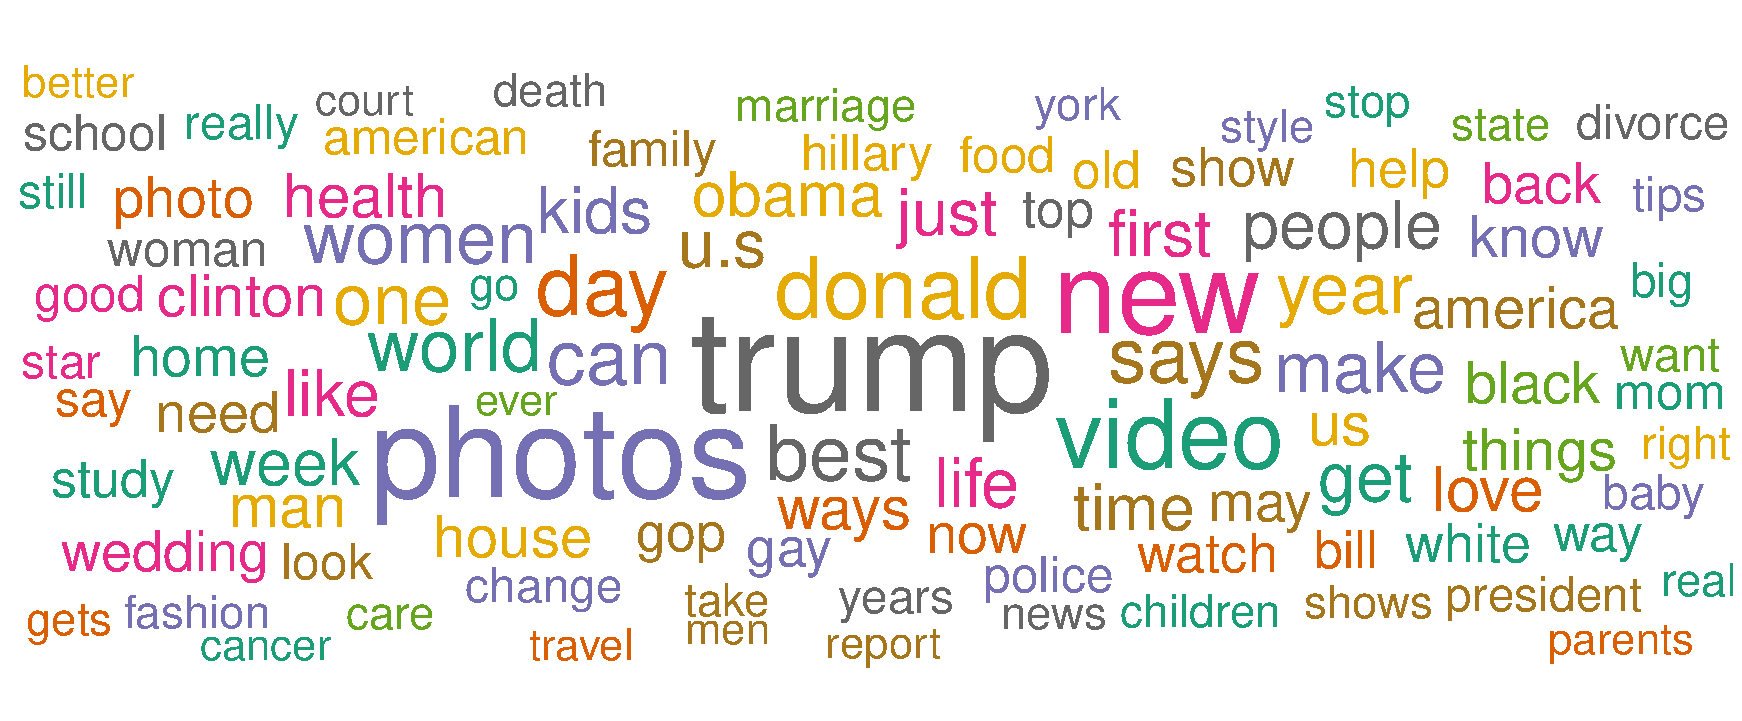
\includegraphics[width = \textwidth,  keepaspectratio]{Images/wordCloudAll.pdf} 
\caption{\textit{Wordcloud} für die häufigsten 100 Wörter aller Kategorien}
\label{abb:WordcloudAll}
\end{figure}


Je größer ein Wort, desto häufiger kommt es insgesamt im Textkorpus vor. Es ist erstaunlich, dass \say{trump} sich über den gesamten Textkorpus als häufigstes Wort etabliert hat, in Anbetracht dessen, dass sich der Zeitraum der Daten auf über $6$ Jahre erstreckt. Die $3$ häufigsten Wörter danach sind \say{photos}, \say{new} und \say{video}. Das überraschend sehr häufige Vorkommen der Wörter \say{photos} und \say{video} könnte ein Indiz dafür sein, dass in einigen Schlagzeilen bereits die Quelle des Medienmaterials angegeben ist, das im Artikel erscheint. Es ist zu sehen, dass viele Namen und Begriffe aus der Politik zu sehen sind, was einleuchtend ist, da \textit{politics} die größte Sparte darstellt. 
Auffallend ist außerdem, dass viele der auftauchenden Begriffe identisch oder fast identisch zu den Namen einiger Kategorien sind. Beispiele dafür sind \say{travel}, \say{wedding}, \say{style} oder \say{parents}. In Abbildung \ref{abb:WordcloudWellness} ist eine weitere \textit{Wordcloud} der zweitgrößten Sparte \textit{wellness \& healthy living} zu sehen.

\begin{figure}[ht]
    \centering
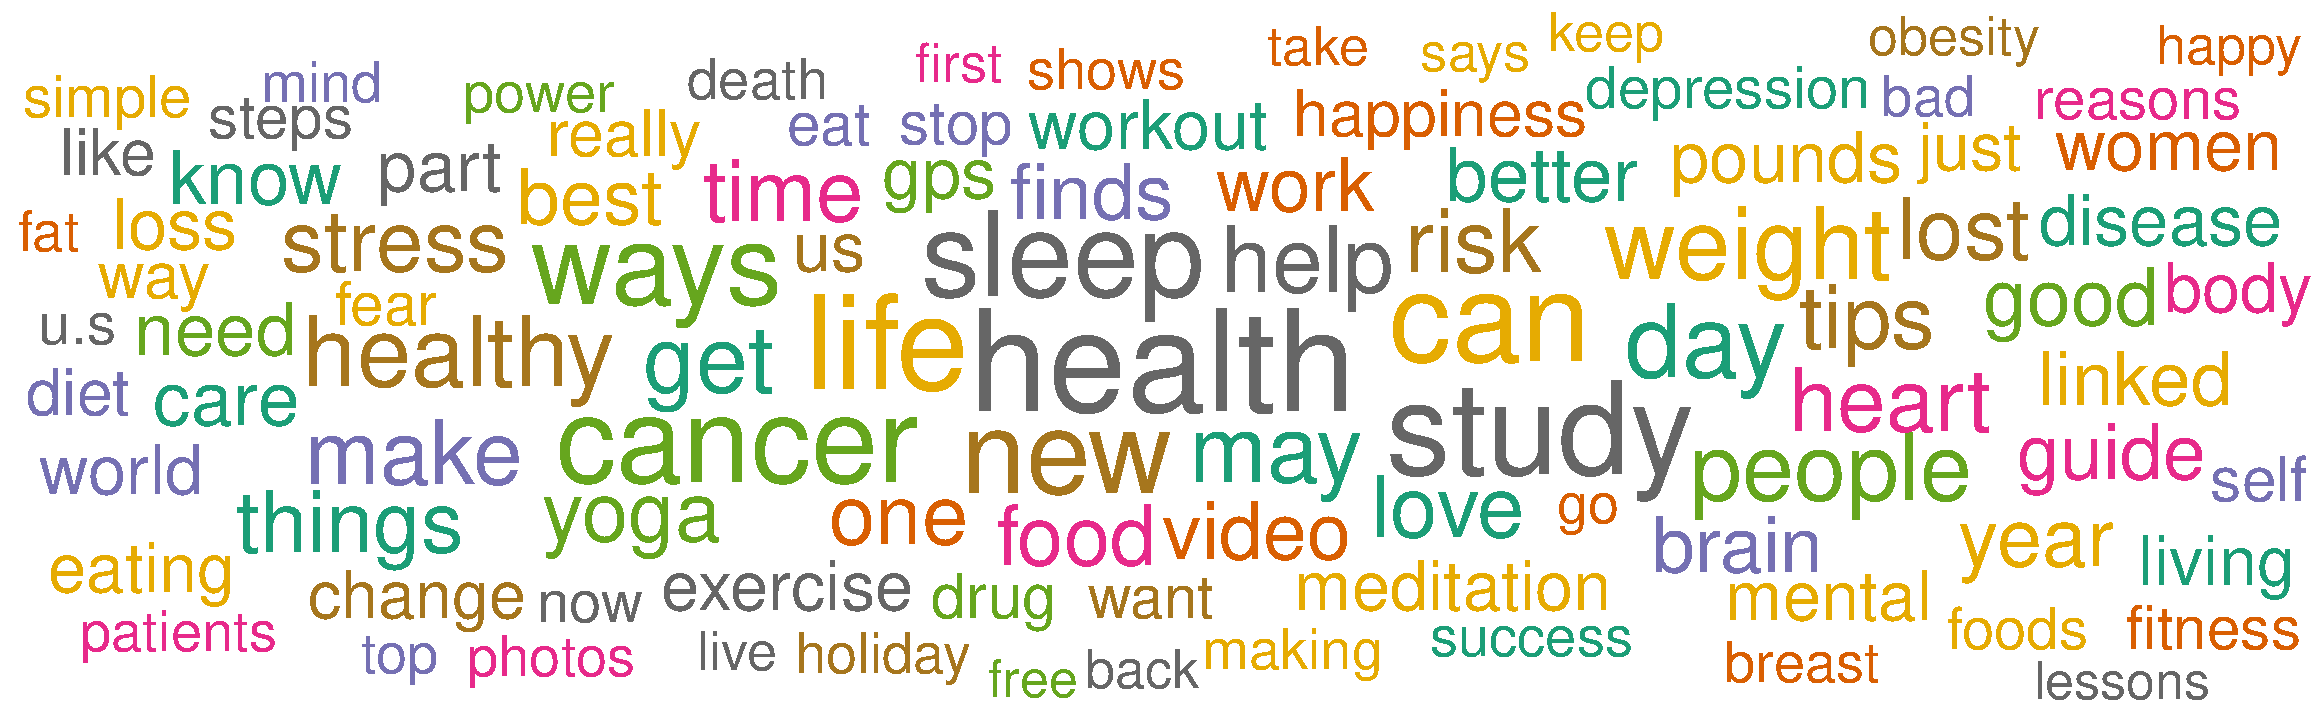
\includegraphics[width = \textwidth,  keepaspectratio]{Images/wordCloudWellness.pdf} 
\caption{\textit{Wordcloud} für die häufigsten 100 Wörter der Kategorie \textit{wellness \& healthy living}}
\label{abb:WordcloudWellness}
\end{figure}

In dieser Kategorie ist zu beobachten, dass oft über Schlaf, Yoga, Meditation und Sport geschrieben wird. Es werden aber auch Krankheiten wie Krebs (\say{cancer}), Übergewichtigkeit (\say{obesity}) und Diabetis angesprochen. \say{yoga}, \say{breast}, \say{diet} oder \say{pounds} könnten auch legitime Schlagwörter für die \say{women} Sparte sein. Genauso ist zu vermuten, dass die Wörter \say{eat}, \say{foods} und \say{healthy} ebenso in \say{food, drink \& taste} oft vorzufinden sind. Mit dem Blick auf die \textit{Wordclouds} und auch in Anbetracht der Zusammenlegung der Kategorien in Kapitel \ref{kap:2_2Aend} fällt auf, dass es nicht immer einfach ist, die Kategorien nur über ihre häufigsten Schlagwörter auseinanderzuhalten. Auf die verschiedenen Möglichkeiten, wie die Schlagzeilen in ein numerisches Datenformat überführt werden können, wird in Kapitel \ref{kap:3.1Wordemb} detailliert eingegangen.
Nachdem nun der Datensatz ausführlich exploriert wurde, folgt im nächsten Unterabschnitt die Zielstellung dieser Thesis.


\subsection{Zielstellung} \label{Kap:Zielst}

Für die Onlinezeitung \textit{Huffpost} kann es von Interesse sein, die Nachrichtensparte eines Artikels unter Vorlage der Schlagzeile automatisch zu kategorisieren. Neben der Kosten- und Zeiteinsparung würden so würden Fehleinschätzungen von Autoren in Form von unpassenden Kategorien vermieden werden.\\
In dieser Thesis wird demnach ein \textit{Multiclass}-Klassifikations\-problem behandelt. Dabei ist die Zielvariable die Nachrichtenkategorie. Diese enthält $32$ Klassen und liegt als Text in kategorieller Form vor. Die in die Modellierung eingehende unabhängige Variable ist die Schlagzeile, welche als numerischer Vektor mit einer der Methoden aus Kapitel \ref{kap:3.1Wordemb} repräsentiert wird. In dieser Problemstellung ist jede Beobachtung genau einer Klasse zugehörig. 

Ziel dieser Arbeit ist es, im Rahmen dieses Klassifikationsproblems verschiedene \textit{Machine-Learning}-Algorithmen auf verschiedenen Arten der Repräsentation der Wörter miteinander zu vergleichen. 

Sei $\bm{x}_i$ die Repräsentation der $i$-ten Beobachtung als Vektor (oder Matrix bei der Repräsentation durch \textit{GloVe}, siehe Kapitel \ref{Kap:Glove}) und $y_i \in \{c_1, ..., c_{32} \}$ die zugehörige Klasse. Die Klassen $\{c_1, ..., c_{32} \}$ können als natürliche Zahlen $\{1, ..., 32 \}$ dargestellt werden.


Für die Vorhersagen $f(\bm{x}_i)$ der trainierten Modelle gilt dann, dass
\begin{center}
$f(\bm{x}_i) = \bm{p}_i = (p(c_1), ...., p(c_{32}))_i$, \hspace{2cm} mit $\sum\limits_{j = 1}^{32} p(c_j) = 1 $,
\end{center}
dabei sind $p(c_j)$, $j = 1,...,32$ die modellierten Wahrscheinlichkeiten der Zugehörigkeit der Beobachtung $\bm{x_i}$ zur Klasse $c_j$, die in Summe $1$ ergeben müssen. Die eindeutige prognostizierte Klasse $\hat{y}$ wird dann zugeordnet durch 
\begin{center}
    $\hat{y} =  \underset{c_1,...,c_{32}}{argmax}$ $p(c_j)$.
\end{center}

Zur Messung der Performance der Modelle erfolgt anhand der Gütemaße aus Kapitel \ref{kap:guetemass} ein Vergleich. 
Es werden Kombinationen aus Repräsentationen der Wörter und verschiedenen Algorithmen im Rahmen einer Vorauswahl getestet. Dabei wird untersucht, welche Repräsentationen der Wörter generell gute Ergebnisse liefern und welche Modelle die bereitgestellte Information am besten nutzen können. Nach der Auswertung der Vorauswahl wird diese auf eine Endauswahl der besten Kombinationen reduziert, auf der alle weiteren Analysen stattfinden.\\
Für diese Endauswahl findet anschließend eine ausführlichere Evaluation statt. Dabei ist nicht nur von Interesse, wie gut die Modelle anhand bestimmter Gütemaße generell abschneiden, sondern auch, ob manche Modelle bestimmte Kategorien trennschärfer identifizieren können. Des Weiteren stellt sich die Frage, in welche Nachbarklassen die Beobachtungen bei einer Fehlklassifikation eingeordnet werden und welche Kategorien die zweit-wahrscheinlichsten sind. Darüber hinaus wird eine Simulation Auskunft darüber geben, wie die Modifikation der Schlagzeilen sich auf die Vorhersagequalität auswirkt. Zuletzt ist es von Interesse, wie die Algorithmen aus den Daten lernen. Dazu wird das Verhalten der Modelle explorativ anhand von $2$ individuellen Schlagzeilen analysiert und erklärt.\\
Im nächsten Abschnitt folgt die Beschreibung der in dieser Arbeit verwendeten statistischen Methoden.


\newpage




\end{document}